% Versão avulsa do exercício 1, para compilar e revisar sozinha (o relatório do grupo usa só exercicio1.tex).
% Antes de compilar, rode na pasta principal:   python exercicio1.py
% Depois, nesta pasta:                          pdflatex exercicio1_avulso.tex   (duas vezes, para as referências)
\documentclass[11pt,a4paper]{article}
\usepackage[utf8]{inputenc}
\usepackage[T1]{fontenc}
\usepackage[brazil]{babel}
\usepackage{amsmath,amssymb}
\usepackage{graphicx}
\usepackage[margin=2.2cm]{geometry}
\usepackage{hyperref}

\graphicspath{{../resultados/}}
% Gerado automaticamente por exercicio1.py. NÃO EDITE À MÃO: rode o script de novo.
\newcommand{\ErroRKRigido}{\ensuremath{9{,}4 \times 10^{-11}}}
\newcommand{\TempoRKRigido}{\ensuremath{21{,}8}\,ms}
\newcommand{\AvalRKRigido}{\ensuremath{884}}
\newcommand{\PassosRKRigido}{\ensuremath{145}}
\newcommand{\ErroRKOscilante}{\ensuremath{6{,}5 \times 10^{-10}}}
\newcommand{\TempoRKOscilante}{\ensuremath{21{,}8}\,ms}
\newcommand{\AvalRKOscilante}{\ensuremath{740}}
\newcommand{\PassosRKOscilante}{\ensuremath{114}}
\newcommand{\ErroRKCoelhos}{\ensuremath{1{,}8 \times 10^{-9}}}
\newcommand{\TempoRKCoelhos}{\ensuremath{54{,}5}\,ms}
\newcommand{\AvalRKCoelhos}{\ensuremath{1.256}}
\newcommand{\PassosRKCoelhos}{\ensuremath{208}}
\newcommand{\ErroPINNRigido}{\ensuremath{9{,}9 \times 10^{-1}}}
\newcommand{\TempoPINNRigido}{\ensuremath{19{,}1}\,s}
\newcommand{\AvalPINNRigido}{\ensuremath{1.000.000}}
\newcommand{\MultaPINNRigido}{\ensuremath{1{,}0}}
\newcommand{\ErroPINNOscilante}{\ensuremath{3{,}9 \times 10^{-4}}}
\newcommand{\TempoPINNOscilante}{\ensuremath{19{,}1}\,s}
\newcommand{\AvalPINNOscilante}{\ensuremath{1.000.000}}
\newcommand{\MultaPINNOscilante}{\ensuremath{6{,}7 \times 10^{-5}}}
\newcommand{\ErroPINNCoelhos}{\ensuremath{9{,}6 \times 10^{-1}}}
\newcommand{\TempoPINNCoelhos}{\ensuremath{25{,}7}\,s}
\newcommand{\AvalPINNCoelhos}{\ensuremath{1.000.000}}
\newcommand{\MultaPINNCoelhos}{\ensuremath{3{,}3 \times 10^{-3}}}
\newcommand{\ErroPINNCoelhosLongo}{\ensuremath{5{,}6 \times 10^{-3}}}
\newcommand{\TempoPINNCoelhosLongo}{\ensuremath{103{,}5}\,s}
\newcommand{\AvalPINNCoelhosLongo}{\ensuremath{4.000.000}}
\newcommand{\MultaPINNCoelhosLongo}{\ensuremath{4{,}2 \times 10^{-6}}}
\newcommand{\ErroPINNRigidoPeso}{\ensuremath{6{,}2 \times 10^{-3}}}
\newcommand{\TempoPINNRigidoPeso}{\ensuremath{19{,}4}\,s}
\newcommand{\AvalPINNRigidoPeso}{\ensuremath{1.000.000}}
\newcommand{\MultaPINNRigidoPeso}{\ensuremath{2{,}0 \times 10^{-2}}}
\newcommand{\ErroPINNRigidoAmarrada}{\ensuremath{1{,}9 \times 10^{-1}}}
\newcommand{\TempoPINNRigidoAmarrada}{\ensuremath{20{,}4}\,s}
\newcommand{\AvalPINNRigidoAmarrada}{\ensuremath{1.000.000}}
\newcommand{\MultaPINNRigidoAmarrada}{\ensuremath{8{,}1}}
\newcommand{\AvalRKMesmoErroRigido}{\ensuremath{134}}
\newcommand{\ErroMelhorPINNRigido}{\ensuremath{6{,}2 \times 10^{-3}}}
\newcommand{\AvalRKMesmoErroOscilante}{\ensuremath{122}}
\newcommand{\ErroMelhorPINNOscilante}{\ensuremath{3{,}9 \times 10^{-4}}}
\newcommand{\AvalRKMesmoErroCoelhos}{\ensuremath{116}}
\newcommand{\ErroMelhorPINNCoelhos}{\ensuremath{5{,}6 \times 10^{-3}}}
\newcommand{\RazaoErroMin}{\ensuremath{6 \times 10^{5}}}
\newcommand{\RazaoErroMax}{\ensuremath{7 \times 10^{7}}}
\newcommand{\RazaoAvalMin}{\ensuremath{1.131}}
\newcommand{\RazaoAvalMax}{\ensuremath{3.185}}
\newcommand{\ToleranciaMinima}{\ensuremath{1 \times 10^{-12}}}
\newcommand{\ToleranciaMaxima}{\ensuremath{1 \times 10^{-3}}}
\newcommand{\DifRefRadau}{\ensuremath{9 \times 10^{-13}}}
\newcommand{\VariacaoInvariante}{\ensuremath{1 \times 10^{-12}}}
\newcommand{\RepeticoesTempoRK}{\ensuremath{20}}
\newcommand{\Semente}{\ensuremath{0}}
\newcommand{\ThreadsTorch}{\ensuremath{6}}
\newcommand{\VersaoTorch}{2.15.0\texttt{+}cpu}
\newcommand{\VersaoScipy}{1.18.1}
   % os números citados no texto, gerados pelo código

\title{PINN versus Runge--Kutta\\\large Exercício 1}
\author{}
\date{}

\begin{document}
\maketitle

% Seção do exercício 1 (versão curta, cerca de 2 páginas), para o relatório do grupo: % Seção do exercício 1 (versão curta, cerca de 2 páginas), para o relatório do grupo: % Seção do exercício 1 (versão curta, cerca de 2 páginas), para o relatório do grupo: \input{exercicio1}.
% Todos os números vêm de ../resultados/numeros.tex e todas as figuras e tabelas de ../resultados/,
% gerados por exercicio1.py: nenhum número é digitado à mão. A versão longa está em exercicio1_completo.tex.

\section{Exercício 1: PINN mínima versus Runge--Kutta adaptativo}

\paragraph{Formulação.} Para $y' = f(t,y)$, $y(a) = y_0$, $t \in [a,b]$, a PINN~\cite{raissi2019} aproxima
$y_\theta(t) = N_\theta(s)$, $s = (t-a)/(b-a)$, com duas camadas ocultas de 32 neurônios ($\tanh$), minimizando
\begin{equation}
  L(\theta) = \frac{1}{N}\sum_{j=1}^{N} \big\| y_\theta'(t_j) - f\big(t_j, y_\theta(t_j)\big) \big\|^2
            + \lambda\, \big\| y_\theta(a) - y_0 \big\|^2
  \label{eq:perda}
\end{equation}
em $N = 200$ pontos de colocação, com $y_\theta'$ por diferenciação automática, Adam (taxa $10^{-3}$), $\lambda = 1$ e
5 mil iterações. O RK45 de Dormand e Prince~\cite{dormand1980} estima o erro local de cada passo pela diferença entre as
soluções de ordens 4 e 5 e ajusta o passo para mantê-lo abaixo de $\mathrm{rtol} = \mathrm{atol} = 10^{-10}$. Nada em
\eqref{eq:perda} controla o erro da solução: ele depende só de quão bem a otimização desce $L$. Comparamos
(i) $y' = -50y$, $y(0) = 1$; (ii) $y' = \cos(20t)$, $y(0) = 0$, ambos em $[0,1]$; e (iii) Lotka--Volterra
$c' = c - cr$, $r' = -r + cr$, $(c,r)(0) = (2,1)$, $t \in [0,10]$, cuja referência é o DOP853 com tolerância
$10^{-13}$ (diferença para o Radau: \DifRefRadau). Seguindo McGreivy e Hakim~\cite{mcgreivy2024}, os dois métodos usam
a mesma régua (erro máximo em 1000 pontos, sobre todas as componentes), o mesmo computador e o mesmo processo, e
traçamos a curva custo $\times$ precisão do RK45 para tolerâncias de \ToleranciaMaxima{} a \ToleranciaMinima. Na PINN,
contamos $N$ avaliações de $f$ por iteração, o que a favorece. A semente é fixada uma única vez.

\begin{table}[ht]
  \centering
  \caption{Erro máximo, tempo e avaliações de $f$.}
  \label{tab:ex1}
  \resizebox{\linewidth}{!}{\input{../resultados/tabela.tex}}
\end{table}

\begin{figure}[ht]
  \centering
  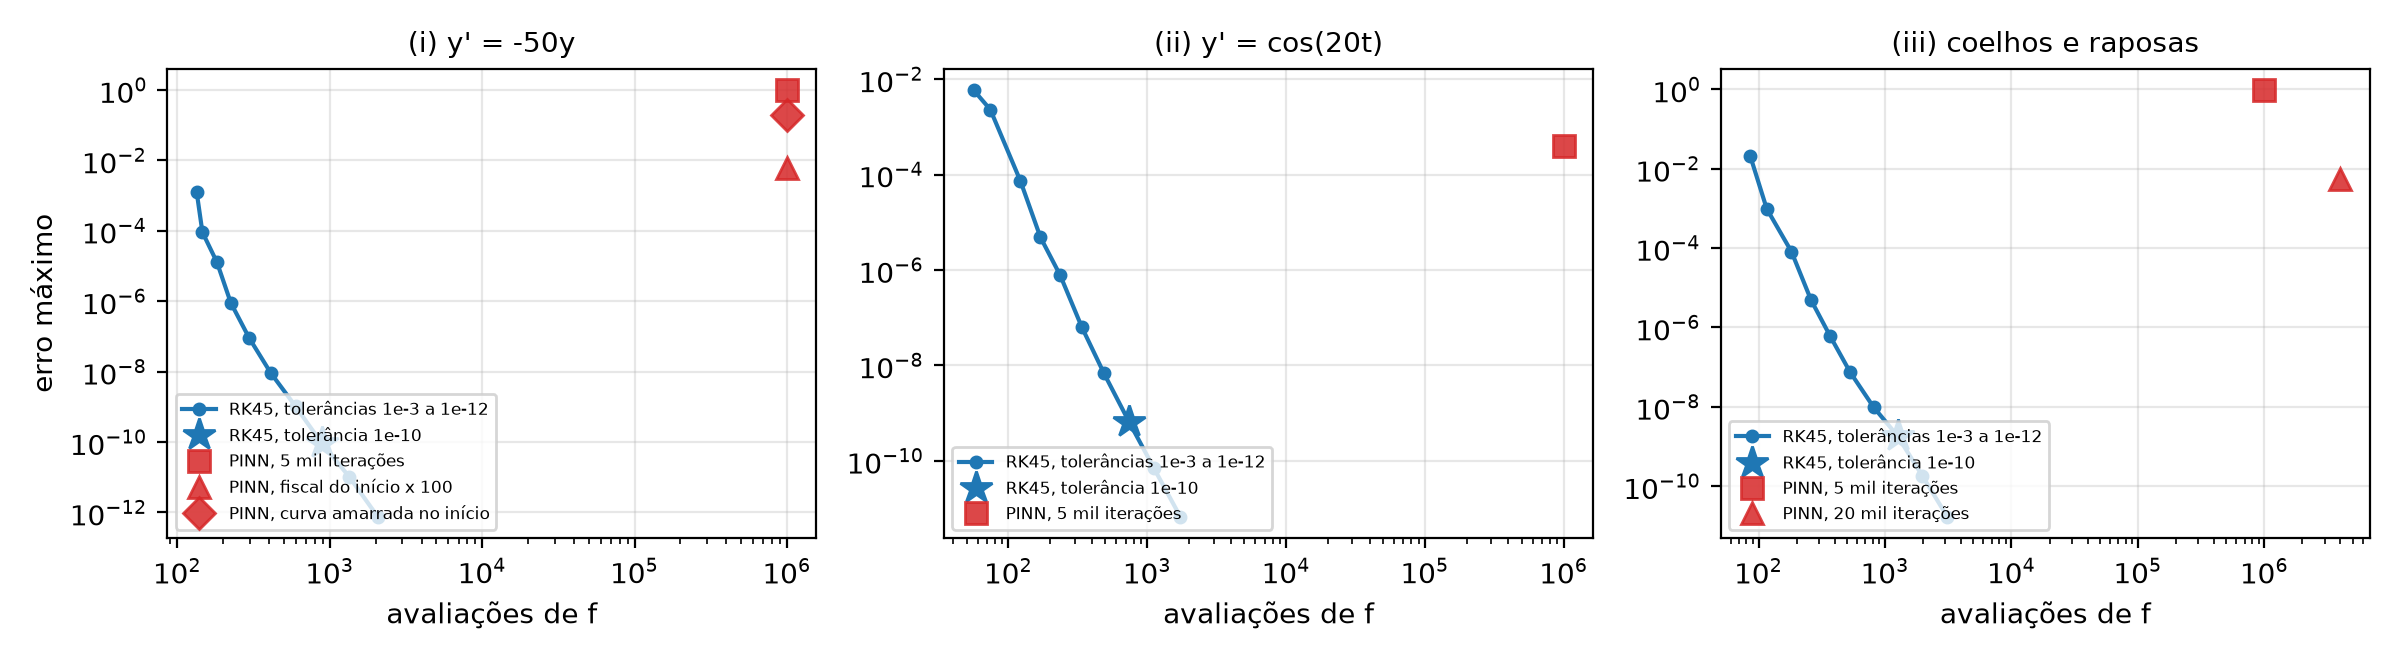
\includegraphics[width=\linewidth]{fig5_custo_compacta.png}
  \caption{Custo $\times$ precisão (abaixo e à esquerda é melhor): curva do RK45 para várias tolerâncias e pontos
  das PINNs.}
  \label{fig:custo}
\end{figure}

\paragraph{Resultados.} A PINN não iguala o RK45 (Tabela~\ref{tab:ex1}, Figura~\ref{fig:custo}). Com 5 mil iterações
(\AvalPINNOscilante{} avaliações), ela falha em (i) e (iii) (erros \ErroPINNRigido{} e \ErroPINNCoelhos) e acerta só
(ii) (\ErroPINNOscilante); o RK45 atinge \ErroRKRigido, \ErroRKOscilante{} e \ErroRKCoelhos{} com no máximo
\AvalRKCoelhos{} avaliações. Mesmo a melhor PINN de cada problema gasta de \RazaoAvalMin{} a \RazaoAvalMax{} vezes mais
avaliações e erra de \RazaoErroMin{} a \RazaoErroMax{} vezes mais; para errar tanto quanto ela, o RK45 precisaria de só
\AvalRKMesmoErroRigido, \AvalRKMesmoErroOscilante{} e \AvalRKMesmoErroCoelhos{} avaliações.

\paragraph{Análise de erro.} \emph{(i) A condição inicial é só uma penalidade.} A constante $y \equiv 0$ tem resíduo
nulo e paga só $L = 1$. Já $y = e^{-kt}$, que respeita $y(0) = 1$, tem resíduo $(50-k)e^{-kt}$ e
$L(k) \approx (50-k)^2/(2k)$, menor que 1 apenas para $k \in (51-\sqrt{101},\, 51+\sqrt{101}) \approx (41, 61)$: fora
dessa faixa estreita, honrar a condição inicial custa mais que ignorá-la, e a otimização para no atalho
($L \approx \MultaPINNRigido$). Com $\lambda = 100$ o erro cai para \ErroPINNRigidoPeso; impondo a condição por
construção, $y_\theta = y_0 + s\,N_\theta(s)$, ela cai só para \ErroPINNRigidoAmarrada, pois a rede tem dificuldade em
representar a queda abrupta. Falha análoga aparece nos problemas de reação rápida de Krishnapriyan et
al.~\cite{krishnapriyan2021} (exercício 2). \emph{(ii) Viés espectral.} A rede aprende primeiro oscilações lentas e só
depois a frequência correta~\cite{rahaman2019}; converge, mas a perda final (\MultaPINNOscilante) é muito menor que o
erro: perda pequena não garante solução precisa. \emph{(iii) Causalidade.} O equilíbrio $(1,1)$ zera o resíduo, como o
zero em (i). Como o resíduo é local, a informação da condição inicial só se propaga durante o treino, da esquerda para
a direita~\cite{wang2024causality}; onde ainda não chegou, a solução se acomoda no equilíbrio. Com 20 mil iterações
(\TempoPINNCoelhosLongo) o erro cai para \ErroPINNCoelhosLongo. O RK45 não sofre de nenhum dos três problemas: controla
o passo e avança no tempo a partir da condição inicial.

\paragraph{Limites e conclusão.} Usamos uma semente, sem ajuste de hiperparâmetros, e o PyTorch em precisão simples
(cerca de 7 algarismos); o RK45 excede um pouco a tolerância no erro global, como esperado de um controle local.
Nenhum desses limites muda a ordem de grandeza da Figura~\ref{fig:custo}. Para problemas de valor inicial bem postos,
a PINN mínima perde do RK45 em custo e em precisão ao mesmo tempo; os problemas inversos e de dados esparsos, em que
ela pode compensar, ficam para o exercício 3.
.
% Todos os números vêm de ../resultados/numeros.tex e todas as figuras e tabelas de ../resultados/,
% gerados por exercicio1.py: nenhum número é digitado à mão. A versão longa está em exercicio1_completo.tex.

\section{Exercício 1: PINN mínima versus Runge--Kutta adaptativo}

\paragraph{Formulação.} Para $y' = f(t,y)$, $y(a) = y_0$, $t \in [a,b]$, a PINN~\cite{raissi2019} aproxima
$y_\theta(t) = N_\theta(s)$, $s = (t-a)/(b-a)$, com duas camadas ocultas de 32 neurônios ($\tanh$), minimizando
\begin{equation}
  L(\theta) = \frac{1}{N}\sum_{j=1}^{N} \big\| y_\theta'(t_j) - f\big(t_j, y_\theta(t_j)\big) \big\|^2
            + \lambda\, \big\| y_\theta(a) - y_0 \big\|^2
  \label{eq:perda}
\end{equation}
em $N = 200$ pontos de colocação, com $y_\theta'$ por diferenciação automática, Adam (taxa $10^{-3}$), $\lambda = 1$ e
5 mil iterações. O RK45 de Dormand e Prince~\cite{dormand1980} estima o erro local de cada passo pela diferença entre as
soluções de ordens 4 e 5 e ajusta o passo para mantê-lo abaixo de $\mathrm{rtol} = \mathrm{atol} = 10^{-10}$. Nada em
\eqref{eq:perda} controla o erro da solução: ele depende só de quão bem a otimização desce $L$. Comparamos
(i) $y' = -50y$, $y(0) = 1$; (ii) $y' = \cos(20t)$, $y(0) = 0$, ambos em $[0,1]$; e (iii) Lotka--Volterra
$c' = c - cr$, $r' = -r + cr$, $(c,r)(0) = (2,1)$, $t \in [0,10]$, cuja referência é o DOP853 com tolerância
$10^{-13}$ (diferença para o Radau: \DifRefRadau). Seguindo McGreivy e Hakim~\cite{mcgreivy2024}, os dois métodos usam
a mesma régua (erro máximo em 1000 pontos, sobre todas as componentes), o mesmo computador e o mesmo processo, e
traçamos a curva custo $\times$ precisão do RK45 para tolerâncias de \ToleranciaMaxima{} a \ToleranciaMinima. Na PINN,
contamos $N$ avaliações de $f$ por iteração, o que a favorece. A semente é fixada uma única vez.

\begin{table}[ht]
  \centering
  \caption{Erro máximo, tempo e avaliações de $f$.}
  \label{tab:ex1}
  \resizebox{\linewidth}{!}{\begin{tabular}{llrrr}
\hline
Problema & Método & Erro máximo & Tempo (s) & Avaliações de f \\
\hline
(i) $y' = -50y$ & RK45, tolerância 1e-10 & 9,39e-11 & 2,18e-02 & 884 \\
(i) $y' = -50y$ & PINN, 5 mil iterações & 9,95e-01 & 1,91e+01 & 1.000.000 \\
(i) $y' = -50y$ & PINN, fiscal do início x 100 & 6,22e-03 & 1,94e+01 & 1.000.000 \\
(i) $y' = -50y$ & PINN, curva amarrada no início & 1,89e-01 & 2,04e+01 & 1.000.000 \\
(ii) $y' = \cos(20t)$ & RK45, tolerância 1e-10 & 6,46e-10 & 2,18e-02 & 740 \\
(ii) $y' = \cos(20t)$ & PINN, 5 mil iterações & 3,91e-04 & 1,91e+01 & 1.000.000 \\
(iii) coelhos e raposas & RK45, tolerância 1e-10 & 1,84e-09 & 5,45e-02 & 1.256 \\
(iii) coelhos e raposas & PINN, 5 mil iterações & 9,63e-01 & 2,57e+01 & 1.000.000 \\
(iii) coelhos e raposas & PINN, 20 mil iterações & 5,59e-03 & 1,04e+02 & 4.000.000 \\
\hline
\end{tabular}
}
\end{table}

\begin{figure}[ht]
  \centering
  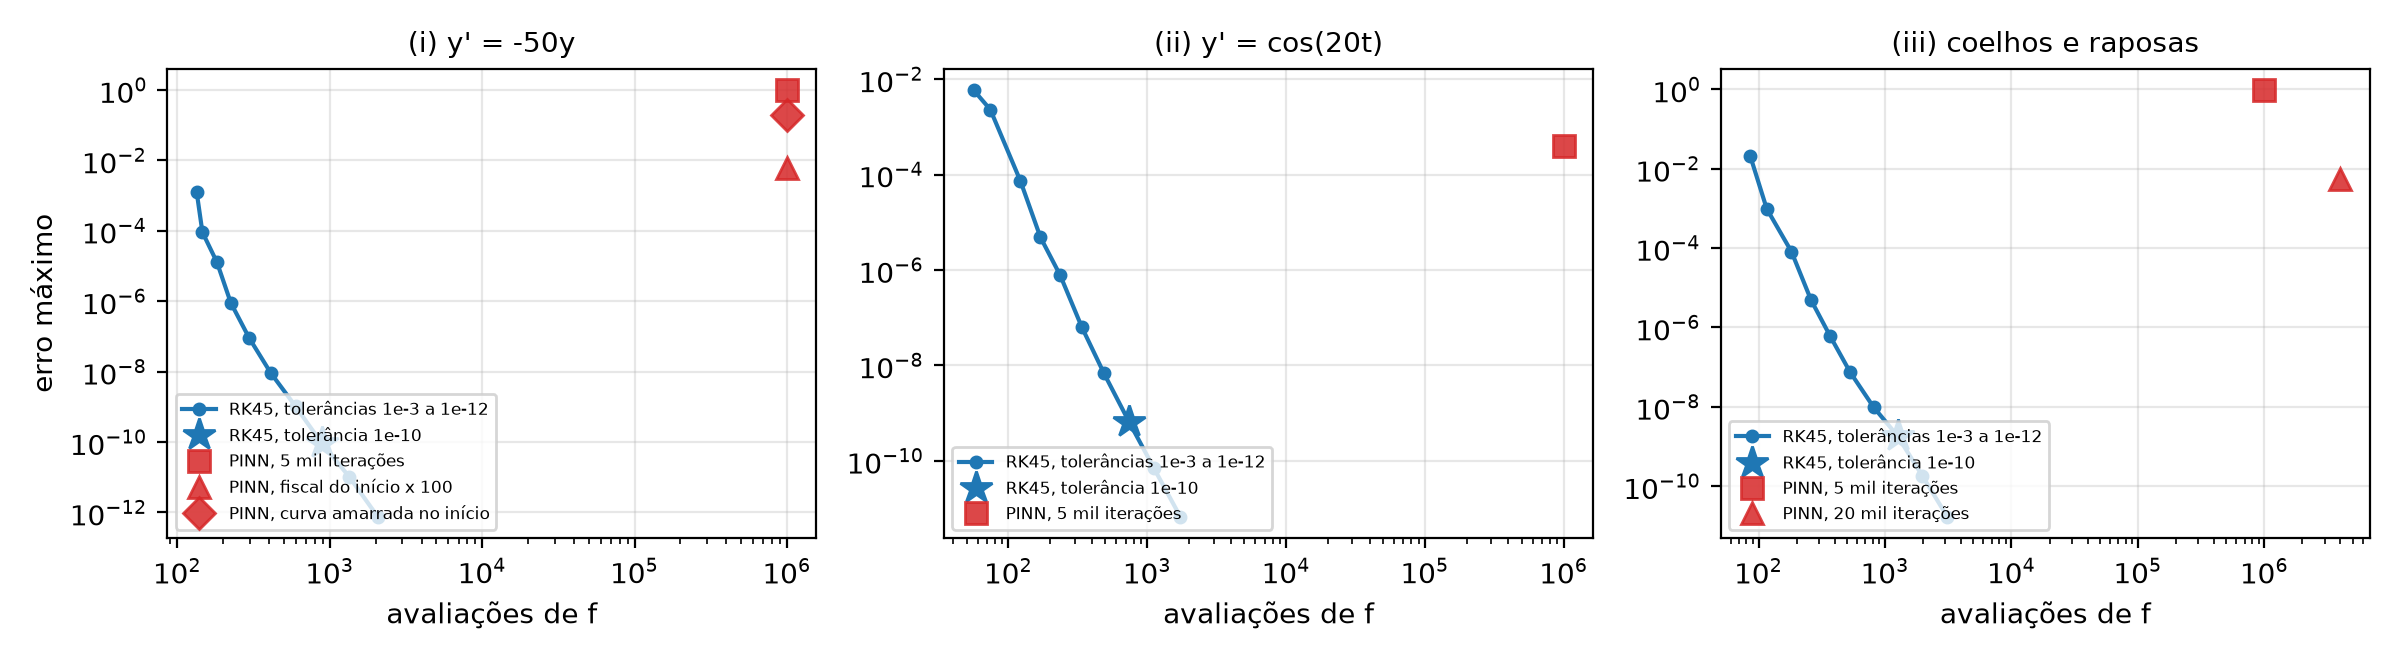
\includegraphics[width=\linewidth]{fig5_custo_compacta.png}
  \caption{Custo $\times$ precisão (abaixo e à esquerda é melhor): curva do RK45 para várias tolerâncias e pontos
  das PINNs.}
  \label{fig:custo}
\end{figure}

\paragraph{Resultados.} A PINN não iguala o RK45 (Tabela~\ref{tab:ex1}, Figura~\ref{fig:custo}). Com 5 mil iterações
(\AvalPINNOscilante{} avaliações), ela falha em (i) e (iii) (erros \ErroPINNRigido{} e \ErroPINNCoelhos) e acerta só
(ii) (\ErroPINNOscilante); o RK45 atinge \ErroRKRigido, \ErroRKOscilante{} e \ErroRKCoelhos{} com no máximo
\AvalRKCoelhos{} avaliações. Mesmo a melhor PINN de cada problema gasta de \RazaoAvalMin{} a \RazaoAvalMax{} vezes mais
avaliações e erra de \RazaoErroMin{} a \RazaoErroMax{} vezes mais; para errar tanto quanto ela, o RK45 precisaria de só
\AvalRKMesmoErroRigido, \AvalRKMesmoErroOscilante{} e \AvalRKMesmoErroCoelhos{} avaliações.

\paragraph{Análise de erro.} \emph{(i) A condição inicial é só uma penalidade.} A constante $y \equiv 0$ tem resíduo
nulo e paga só $L = 1$. Já $y = e^{-kt}$, que respeita $y(0) = 1$, tem resíduo $(50-k)e^{-kt}$ e
$L(k) \approx (50-k)^2/(2k)$, menor que 1 apenas para $k \in (51-\sqrt{101},\, 51+\sqrt{101}) \approx (41, 61)$: fora
dessa faixa estreita, honrar a condição inicial custa mais que ignorá-la, e a otimização para no atalho
($L \approx \MultaPINNRigido$). Com $\lambda = 100$ o erro cai para \ErroPINNRigidoPeso; impondo a condição por
construção, $y_\theta = y_0 + s\,N_\theta(s)$, ela cai só para \ErroPINNRigidoAmarrada, pois a rede tem dificuldade em
representar a queda abrupta. Falha análoga aparece nos problemas de reação rápida de Krishnapriyan et
al.~\cite{krishnapriyan2021} (exercício 2). \emph{(ii) Viés espectral.} A rede aprende primeiro oscilações lentas e só
depois a frequência correta~\cite{rahaman2019}; converge, mas a perda final (\MultaPINNOscilante) é muito menor que o
erro: perda pequena não garante solução precisa. \emph{(iii) Causalidade.} O equilíbrio $(1,1)$ zera o resíduo, como o
zero em (i). Como o resíduo é local, a informação da condição inicial só se propaga durante o treino, da esquerda para
a direita~\cite{wang2024causality}; onde ainda não chegou, a solução se acomoda no equilíbrio. Com 20 mil iterações
(\TempoPINNCoelhosLongo) o erro cai para \ErroPINNCoelhosLongo. O RK45 não sofre de nenhum dos três problemas: controla
o passo e avança no tempo a partir da condição inicial.

\paragraph{Limites e conclusão.} Usamos uma semente, sem ajuste de hiperparâmetros, e o PyTorch em precisão simples
(cerca de 7 algarismos); o RK45 excede um pouco a tolerância no erro global, como esperado de um controle local.
Nenhum desses limites muda a ordem de grandeza da Figura~\ref{fig:custo}. Para problemas de valor inicial bem postos,
a PINN mínima perde do RK45 em custo e em precisão ao mesmo tempo; os problemas inversos e de dados esparsos, em que
ela pode compensar, ficam para o exercício 3.
.
% Todos os números vêm de ../resultados/numeros.tex e todas as figuras e tabelas de ../resultados/,
% gerados por exercicio1.py: nenhum número é digitado à mão. A versão longa está em exercicio1_completo.tex.

\section{Exercício 1: PINN mínima versus Runge--Kutta adaptativo}

\paragraph{Formulação.} Para $y' = f(t,y)$, $y(a) = y_0$, $t \in [a,b]$, a PINN~\cite{raissi2019} aproxima
$y_\theta(t) = N_\theta(s)$, $s = (t-a)/(b-a)$, com duas camadas ocultas de 32 neurônios ($\tanh$), minimizando
\begin{equation}
  L(\theta) = \frac{1}{N}\sum_{j=1}^{N} \big\| y_\theta'(t_j) - f\big(t_j, y_\theta(t_j)\big) \big\|^2
            + \lambda\, \big\| y_\theta(a) - y_0 \big\|^2
  \label{eq:perda}
\end{equation}
em $N = 200$ pontos de colocação, com $y_\theta'$ por diferenciação automática, Adam (taxa $10^{-3}$), $\lambda = 1$ e
5 mil iterações. O RK45 de Dormand e Prince~\cite{dormand1980} estima o erro local de cada passo pela diferença entre as
soluções de ordens 4 e 5 e ajusta o passo para mantê-lo abaixo de $\mathrm{rtol} = \mathrm{atol} = 10^{-10}$. Nada em
\eqref{eq:perda} controla o erro da solução: ele depende só de quão bem a otimização desce $L$. Comparamos
(i) $y' = -50y$, $y(0) = 1$; (ii) $y' = \cos(20t)$, $y(0) = 0$, ambos em $[0,1]$; e (iii) Lotka--Volterra
$c' = c - cr$, $r' = -r + cr$, $(c,r)(0) = (2,1)$, $t \in [0,10]$, cuja referência é o DOP853 com tolerância
$10^{-13}$ (diferença para o Radau: \DifRefRadau). Seguindo McGreivy e Hakim~\cite{mcgreivy2024}, os dois métodos usam
a mesma régua (erro máximo em 1000 pontos, sobre todas as componentes), o mesmo computador e o mesmo processo, e
traçamos a curva custo $\times$ precisão do RK45 para tolerâncias de \ToleranciaMaxima{} a \ToleranciaMinima. Na PINN,
contamos $N$ avaliações de $f$ por iteração, o que a favorece. A semente é fixada uma única vez.

\begin{table}[ht]
  \centering
  \caption{Erro máximo, tempo e avaliações de $f$.}
  \label{tab:ex1}
  \resizebox{\linewidth}{!}{\begin{tabular}{llrrr}
\hline
Problema & Método & Erro máximo & Tempo (s) & Avaliações de f \\
\hline
(i) $y' = -50y$ & RK45, tolerância 1e-10 & 9,39e-11 & 2,18e-02 & 884 \\
(i) $y' = -50y$ & PINN, 5 mil iterações & 9,95e-01 & 1,91e+01 & 1.000.000 \\
(i) $y' = -50y$ & PINN, fiscal do início x 100 & 6,22e-03 & 1,94e+01 & 1.000.000 \\
(i) $y' = -50y$ & PINN, curva amarrada no início & 1,89e-01 & 2,04e+01 & 1.000.000 \\
(ii) $y' = \cos(20t)$ & RK45, tolerância 1e-10 & 6,46e-10 & 2,18e-02 & 740 \\
(ii) $y' = \cos(20t)$ & PINN, 5 mil iterações & 3,91e-04 & 1,91e+01 & 1.000.000 \\
(iii) coelhos e raposas & RK45, tolerância 1e-10 & 1,84e-09 & 5,45e-02 & 1.256 \\
(iii) coelhos e raposas & PINN, 5 mil iterações & 9,63e-01 & 2,57e+01 & 1.000.000 \\
(iii) coelhos e raposas & PINN, 20 mil iterações & 5,59e-03 & 1,04e+02 & 4.000.000 \\
\hline
\end{tabular}
}
\end{table}

\begin{figure}[ht]
  \centering
  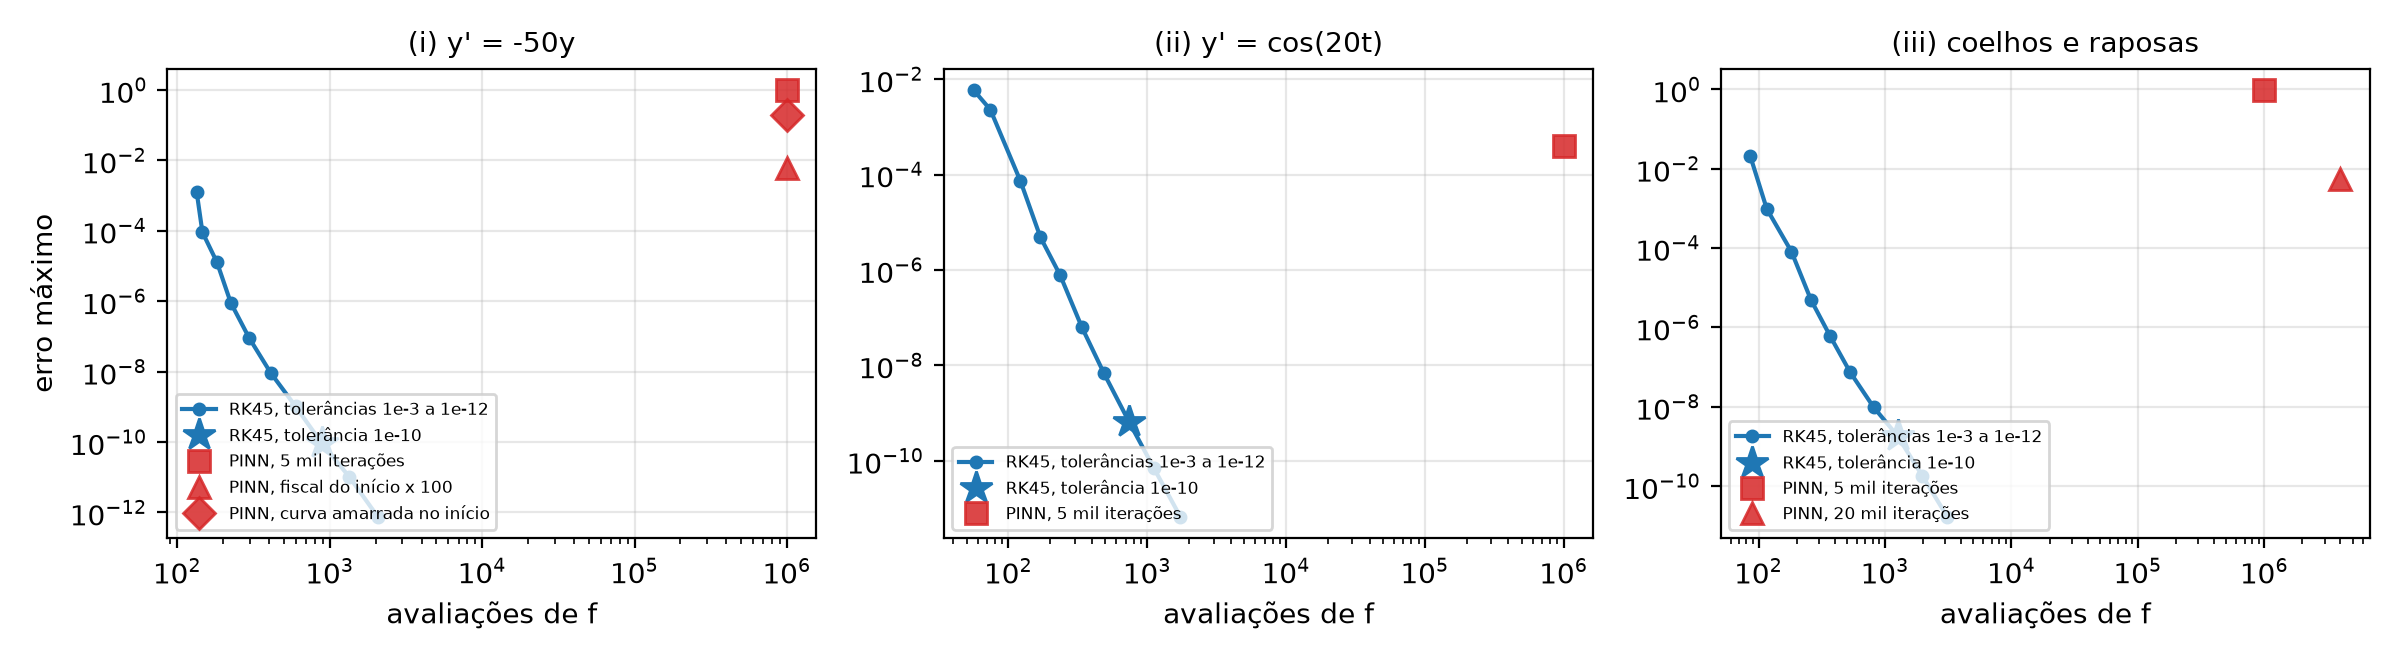
\includegraphics[width=\linewidth]{fig5_custo_compacta.png}
  \caption{Custo $\times$ precisão (abaixo e à esquerda é melhor): curva do RK45 para várias tolerâncias e pontos
  das PINNs.}
  \label{fig:custo}
\end{figure}

\paragraph{Resultados.} A PINN não iguala o RK45 (Tabela~\ref{tab:ex1}, Figura~\ref{fig:custo}). Com 5 mil iterações
(\AvalPINNOscilante{} avaliações), ela falha em (i) e (iii) (erros \ErroPINNRigido{} e \ErroPINNCoelhos) e acerta só
(ii) (\ErroPINNOscilante); o RK45 atinge \ErroRKRigido, \ErroRKOscilante{} e \ErroRKCoelhos{} com no máximo
\AvalRKCoelhos{} avaliações. Mesmo a melhor PINN de cada problema gasta de \RazaoAvalMin{} a \RazaoAvalMax{} vezes mais
avaliações e erra de \RazaoErroMin{} a \RazaoErroMax{} vezes mais; para errar tanto quanto ela, o RK45 precisaria de só
\AvalRKMesmoErroRigido, \AvalRKMesmoErroOscilante{} e \AvalRKMesmoErroCoelhos{} avaliações.

\paragraph{Análise de erro.} \emph{(i) A condição inicial é só uma penalidade.} A constante $y \equiv 0$ tem resíduo
nulo e paga só $L = 1$. Já $y = e^{-kt}$, que respeita $y(0) = 1$, tem resíduo $(50-k)e^{-kt}$ e
$L(k) \approx (50-k)^2/(2k)$, menor que 1 apenas para $k \in (51-\sqrt{101},\, 51+\sqrt{101}) \approx (41, 61)$: fora
dessa faixa estreita, honrar a condição inicial custa mais que ignorá-la, e a otimização para no atalho
($L \approx \MultaPINNRigido$). Com $\lambda = 100$ o erro cai para \ErroPINNRigidoPeso; impondo a condição por
construção, $y_\theta = y_0 + s\,N_\theta(s)$, ela cai só para \ErroPINNRigidoAmarrada, pois a rede tem dificuldade em
representar a queda abrupta. Falha análoga aparece nos problemas de reação rápida de Krishnapriyan et
al.~\cite{krishnapriyan2021} (exercício 2). \emph{(ii) Viés espectral.} A rede aprende primeiro oscilações lentas e só
depois a frequência correta~\cite{rahaman2019}; converge, mas a perda final (\MultaPINNOscilante) é muito menor que o
erro: perda pequena não garante solução precisa. \emph{(iii) Causalidade.} O equilíbrio $(1,1)$ zera o resíduo, como o
zero em (i). Como o resíduo é local, a informação da condição inicial só se propaga durante o treino, da esquerda para
a direita~\cite{wang2024causality}; onde ainda não chegou, a solução se acomoda no equilíbrio. Com 20 mil iterações
(\TempoPINNCoelhosLongo) o erro cai para \ErroPINNCoelhosLongo. O RK45 não sofre de nenhum dos três problemas: controla
o passo e avança no tempo a partir da condição inicial.

\paragraph{Limites e conclusão.} Usamos uma semente, sem ajuste de hiperparâmetros, e o PyTorch em precisão simples
(cerca de 7 algarismos); o RK45 excede um pouco a tolerância no erro global, como esperado de um controle local.
Nenhum desses limites muda a ordem de grandeza da Figura~\ref{fig:custo}. Para problemas de valor inicial bem postos,
a PINN mínima perde do RK45 em custo e em precisão ao mesmo tempo; os problemas inversos e de dados esparsos, em que
ela pode compensar, ficam para o exercício 3.


\begin{thebibliography}{9}
\bibitem{raissi2019} M. Raissi, P. Perdikaris e G. E. Karniadakis. Physics-informed neural networks: a deep learning
  framework for solving forward and inverse problems involving nonlinear partial differential equations.
  \emph{Journal of Computational Physics}, 378:686--707, 2019.
\bibitem{dormand1980} J. R. Dormand e P. J. Prince. A family of embedded Runge--Kutta formulae.
  \emph{Journal of Computational and Applied Mathematics}, 6(1):19--26, 1980.
\bibitem{mcgreivy2024} N. McGreivy e A. Hakim. Weak baselines and reporting biases lead to overoptimism in machine
  learning for fluid-related partial differential equations. \emph{Nature Machine Intelligence}, 6:1256--1269, 2024.
\bibitem{rahaman2019} N. Rahaman et al. On the spectral bias of neural networks. \emph{Proceedings of the 36th
  International Conference on Machine Learning (ICML)}, 2019.
\bibitem{wang2024causality} S. Wang, S. Sankaran e P. Perdikaris. Respecting causality for training physics-informed
  neural networks. \emph{Computer Methods in Applied Mechanics and Engineering}, 421:116813, 2024.
\bibitem{krishnapriyan2021} A. S. Krishnapriyan, A. Gholami, S. Zhe, R. M. Kirby e M. W. Mahoney. Characterizing
  possible failure modes in physics-informed neural networks. \emph{Advances in Neural Information Processing Systems
  (NeurIPS)}, 34, 2021.
\end{thebibliography}

\end{document}
